\documentclass{report}
    \title{\textbf{CEN4010 - Notes}}
    \author{William L. Thomson Jr.}
    \date{Spring Semester 2022}
    \usepackage[tmargin=1in,lmargin=1in,rmargin=1in,bmargin=1in]{geometry}
    \usepackage[dvipsnames]{xcolor}
	\usepackage{enumitem}
    \usepackage[T1]{fontenc}
	\usepackage{hyperref}
    \usepackage{float}
    \usepackage{graphicx}
    \usepackage{makecell}
    \usepackage{multicol, caption}
	\usepackage{titlesec}
    \renewcommand{\familydefault}{\sfdefault}        	 
    \renewcommand\theadfont{\bfseries\sffamily}
    
	\hypersetup{ colorlinks=true, linkcolor=blue, filecolor=purple, urlcolor=cyan }

    \titleformat{\chapter}
	{\Large\bfseries}
	{\thechapter.}{0.5em}{}
	
	\titleformat{\section}
	{\large\bfseries}
	{\thesection.}{0.5em}{}
	
	\titleformat{\subsection}
	{\normalsize\bfseries}
	{\thesection.}{0.5em}{}

    \titlespacing\chapter{0pt}{12pt plus 0pt minus 4pt}{0pt plus 0pt minus 4pt}
    \titlespacing\section{0pt}{12pt plus 4pt minus 8pt}{0pt plus 2pt minus 8pt}
    \titlespacing\subsection{0pt}{12pt plus 4pt minus 4pt}{0pt plus 2pt minus 4pt}
    \titlespacing\subsubsection{0pt}{12pt plus 4pt minus 2pt}{0pt plus 2pt minus 2pt}

    \setlist[description]{noitemsep, topsep=0pt, itemsep=-.1em}
    \setlist[enumerate]{noitemsep, topsep=0pt, itemsep=-.1em}
    \setlist[itemize]{noitemsep, topsep=0pt, itemsep=-.1em}
    \setlist[trivlist]{noitemsep, topsep=-8pt, itemsep=-.1em}
	
    \newcommand{\comment}[1]{}
    \newcommand{\textr}[1]{\textcolor{red}{#1}}
    \newcommand{\textg}[1]{\textcolor{ForestGreen}{#1}}
    \newcommand{\textv}[1]{\textcolor{violet}{#1}}
    \newcommand{\textbfr}[1]{\textbf{\textr{#1}}}
    \newcommand{\textbfg}[1]{\textbf{\textg{#1}}}
    \newcommand{\textbfv}[1]{\textbf{\textv{#1}}}
\begin{document}

\maketitle
\tableofcontents
\newpage

\chapter{Professional Software Development}
\section{Software engineering}
\begin{itemize}
  \item Software engineering is an engineering discipline that is concerned with all aspects of software production from the early stages of system specification through to maintaining the system after it has gone into use. (Note: professor definition)
  \item Engineering discipline
  \begin{itemize}
    \item Using appropriate theories \& methods to solve problems bearing in mind
organizational \& financial constraints
\end{itemize}
  \item All aspects of software production
  \begin{itemize}
    \item Not just technical process of development
    \item Also project management \& the development of tools, methods etc. to support software production
  \end{itemize}
  \item The economies of ALL nations are dependent on software.
  \item More \& more systems are software controlled.
  \item Software engineering is concerned with theories, methods \& tools for professional software development.
  \item Expenditure on software represents a significant fraction of GNP/GDP in all developed countries
\end{itemize}

\section{Software costs}
\begin{itemize}
  \item Software costs often dominate computer system costs. The costs of software on a PC are often greater than the hardware cost.
  \item Software costs more to maintain than it does to develop. For systems with a long life, maintenance costs may be several times higher than the development costs.
  \item Software engineering is concerned with cost-effective software development.
\end{itemize}

\section{Software products - Generic vs Customized}
\noindent \textbf{Generic products} \newline
The specification of what the software should do is owned by the software developer \& decisions on software change are made by the developer.
    \begin{itemize}
      \item Stand-alone systems that are marketed \& sold to any customer who
wishes to buy them.
      \item Examples
        \begin{itemize}
          \item PC software such as graphics programs
          \item Project management tools
          \item CAD software
          \item Software for specific markets such as appointments systems for dentists.
        \end{itemize}
    \end{itemize}
\noindent \textbf{Customized products} \newline
The specification of what the software should do is owned by the customer for the software \& they make decisions on software changes that are required.
    \begin{itemize}
      \item Software that is commissioned by a specific customer to meet their own needs.
      \item Examples – embedded control systems, air traffic control software, traffic monitoring systems.
    \end{itemize}
    
\section{Quality/Essential attributes of good software}
\noindent \textbf{Maintainability}\newline
Software should be written in such a way so that it can evolve to meet the changing needs of customers. This is a critical attribute because software change is an inevitable requirement of a changing business environment.\newline
\textbf{Dependability \& security}\newline
Software dependability includes a range of characteristics including reliability, security \& safety. Dependable software should not cause physical or economic damage in the event of
system failure. Malicious users should not be able to access or damage the system\newline
\textbf{Efficiency}\newline
Software should not make wasteful use of system resources such as memory \& processor cycles. Efficiency therefore includes responsiveness, processing time, memory utilization, etc\newline
\textbf{Acceptability}\newline
Software must be acceptable to the type of users for which it is designed. This means that it must be understandable, usable \& compatible with other systems that they use.

\newpage
\section{Frequently asked questions about software engineering}
\noindent \textbf{What is software?}\newline
  Computer programs \& associated documentation. Software products may be developed for a particular customer or may be developed for a general market.
\newline\newline
\textbf{What are the attributes of good software?}\newline
  Good software should deliver the required functionality \& performance to the user \& should be maintainable, dependable \& usable.
\newline\newline
\textbf{What is software engineering?}\newline
Software engineering is an engineering discipline that is
concerned with all aspects of software production
\newline\newline
\textbf{What are the fundamental software engineering activities?}\newline
Software specification, software development, software
validation \& software evolution(maintenance)
\newline\newline
\textbf{What are the key challenges facing software engineering?}\newline
Coping with increasing diversity, demands for reduced delivery times \& developing trustworthy software.
\newline\newline
\textbf{What are the costs of software engineering?}\newline
Roughly 60\% of software costs are development costs, 40\% are testing costs. For custom software, evolution costs often exceed development costs.
\newline\newline
\textbf{What are the best software engineering techniques \& methods?}\newline
While all software projects have to be professionally managed \& developed, different techniques are appropriate for different types of system. For example, games should always be developed using a series of prototypes whereas safety critical control systems require a complete \& analyzable specification to be developed. You can’t, therefore, say that one method is better than another.

\subsection{Computer Science vs Software Engineering}
\noindent\textbf{What is the difference between software engineering \& computer science?}\newline
Computer science focuses on theory \& fundamentals; software engineering is concerned with the practicalities of developing \& delivering useful software.

\subsection{Software Engineering vs Systems Engineering}
\noindent\textbf{What is the difference between software engineering \& system engineering?}\newline
System engineering is concerned with all aspects of computer-based systems development including hardware, software \& process engineering. Software engineering is part of this more general process

\subsection{World Wide Web}
\noindent\textbf{What differences has the web made to software engineering?}\newline
The web has led to the availability of software services \& the possibility of developing highly distributed service-based systems. Web-based systems development has led to important advances in programming languages \& software reuse.

\newpage
\section{Fundamental Software Process Activities}
\begin{description}[style=multiline,leftmargin=12em]
  \item [\textr{Software specification}] where customers \& engineers
define the software that is to be produced \& the constraints on its operation.
  \item [\textr{Software development}] where the software is designed \& programmed.
  \item [\textr{Software validation}] where the software is checked to ensure that it is what the customer requires.
  \item [\textr{Software evolution}] where the software is modified to reflect changing customer \& market requirements.
\end{description}

\section{Application types}
\begin{description}
  \item [Stand-alone applications] \
  \begin{itemize}
    \item These are application systems that run on a local computer, such as a PC.
    \item They include all necessary functionality \& do not need to be connected to a
network.
  \end{itemize}
  \item [Interactive transaction-based applications] \
  \begin{itemize}
    \item Applications that execute on remote computer \& accessed by users from
their own PCs or terminals.
	\item These include web applications such as e-commerce applications.
  \end{itemize}
  \item [Embedded control systems] \
  \begin{itemize}
    \item These are software control systems that control \& manage hardware devices.
    \item Numerically, there are probably more embedded systems than any other type of
system.
  \end{itemize}
  \item [Batch processing systems] \
  \begin{itemize}
    \item These are business systems that are designed to process data in
large batches.
    \item They process large numbers of individual inputs to create
corresponding outputs.
  \end{itemize}
  \item [Entertainment systems] \
  \begin{itemize}
    \item These are systems that are primarily for personal use \& which
are intended to entertain the user.
  \end{itemize}
  \item [Systems for modeling \& simulation] \
  \begin{itemize}
    \item These are systems that are developed by scientists \& engineers
to model physical processes or situations, which include many,
separate, interacting objects.
  \end{itemize}
  \item [Data collection systems] \
  \begin{itemize}
    \item These are systems that collect data from their environment using a
set of sensors \& send that data to other systems for processing.
  \end{itemize}
  \item [Systems of systems] \ \newline
These are systems that are composed of a number of other software systems.
\end{description}

\section{Software Engineering Ethics}
\begin{itemize}
  \item Software engineering involves wider responsibilities than simply the application of technical skills
  \item Software engineering must behave in an honest \& ethically responsible way to be respected as professionals.
  \item Ethical behavior is more than upholding the law it involves following principles that are morally correct.
  \item Software engineers have a moral obligation to build reliable software that does no harm to other people
\end{itemize}

\section{Issues of professional responsibility}
\begin{description}[style=multiline,leftmargin=8em]
  \item [Confidentiality] Engineers should normally respect the confidentiality of their employers or clients irrespective of whether or not a formal confidentiality agreement has been signed.
  \item [Competence] Engineers should not misrepresent their level of competence. They should not knowingly accept work which is outwith their competence.
\end{description}
\begin{description}
  \item [Intellectual Property Rights] \
  \begin{itemize}
    \item Engineers should be aware of local laws governing use of intellectual property; patents, copyright, etc.
    \item They should be careful to ensure that the intellectual property of employers \& clients is protected.
  \end{itemize}
  \item [Intellectual Property Rights] \
  \begin{itemize}
    \item Software engineers should not use their technical skills to misuse other people's computers
    \item Computer misuse ranges from relatively trivial (game playing on an employer's machine to extremely serious (dissemination of virus)
  \end{itemize}
\end{description}

\section{ACM/IEEE Code of Ethics}
\begin{itemize}
  \item The professional societies in the US have cooperated to produce a good code of ethical practices
  \item Members of these organizations sign up to the code of practice when they join.
  \item The Code contains eight Principles related to the behavior of \& decisions made by professional software engineers, including practitioners, educators, managers, supervisors, \& policy makers, as well as trainees \& students of the profession.
\end{itemize}



%------------------------------------- Requirements Engineering ----------------------------------
\newpage
\chapter{Requirements Engineering}
\section{Requirements Engineering (RE)}
\noindent Requirements Engineering (RE) is a \textbf{set of activities} concerned with \textbf{identifying \& communicating} the \textbf{purpose} of a software-intensive system, \& the \textbf{contexts} in which it will be used. Hence, RE acts as the bridge between the \textbf{real world needs} of users, customers, \& other \textbf{constituencies} affected by a software system \& the \textbf{capabilities \& opportunities} afforded by software-intensive technologies
\begin{itemize}
  \item Discovering stakeholder goals, needs, \& expectations
  \item Communicating these to system implementers
\end{itemize}

\section{Requirements}
\noindent Stake holders needs \& desires\newline
\textbf{Requirement IEEE Definition:}
  \begin{itemize}
    \item a condition or capability needed by a user to solve a \textbfr{problem} or achieve an objective
    \item a condition or capability that must be met or possessed by a system or system component to satisfy a contract, standard, specification, or other formally imposed document
  \end{itemize}
A \textbf{problem} is a difference between things as desired \& things as perceived

\subsection{Types of Requirements}
\begin{description}
  \item [User requirements] - Written for customers\newline
  Statements in natural language plus diagrams of services the system provides \& its operational constraints.\newline
  \textbf{Readers:} Client manager, System end-users, Client engineers, Contract managers, System architect
  \item [System requirements] - Written as a contract between client \& contractor \newline
  A structured document setting out detailed descriptions of the system services.\newline
  \textbf{Readers:} System end-users, Client engineers, System architects, Software developers
  \item [Software specification] - Written for developers \newline
  A detailed software description which can serve as a basis for a design or implementation. \newline
  \textbf{Readers:} Client engineers (perhaps), System architects, Software developers
\end{description}

\subsection{Functional \& Non-Functional Requirements}
\begin{description}
  \item [Functional requirements] \ \newline
   Statements of services the system should provide, how the system should react to particular inputs \& how the system should behave in particular situations. (Specific details/specs of the function of the software)
  \item [Non-Functional requirements] \ \newline
   Constraints on the services or functions offered by the system such as timing constraints, constraints on the development process, standards, etc. Ex: Security, Extensibility, Scalability, Portability etc
\end{description}
\begin{figure}[H]
\centering
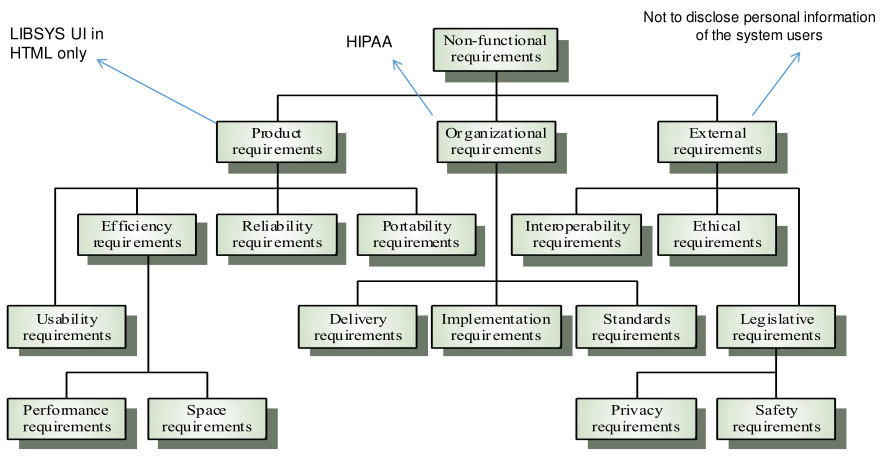
\includegraphics[scale=.45,trim=1cm 1cm 1cm 1cm]{assets/CEN4010_Non-Function_Requirements.jpg}
\end{figure}


\subsection{The meaning of requirements}
\begin{description}[style=multiline,leftmargin=9.5em]
  \item [Domain Properties] Things in the \textbfr{application domain} that are true regardless if we ever build  proposed system
  \item [Requirements] Things in the \textbfr{application domain} we wish to be made true by delivering proposed system\newline
Many of which will involve phenomena to which the machine has no
access
  \item [A Specification] Description of behaviors that the \textbfr{program} must have in order to meet the \textbfr{requirements}\newline 
Can only be written in terms of shared phenomena!
\end{description}

\section{Importance of RE}
\vspace{-1em}
\begin{multicols}{2}
\textbf{Problems}
\begin{itemize}
  \item Increased reliance on software
  \item Software biggest cost for mission critical systems
  \item Wastage on failed projects
\end{itemize}
\textbf{Key Factors}
\begin{itemize}
  \item Certification costs
  \item Re-work from defect removal
  \item Changing requirements
\end{itemize}
\end{multicols}

\section{Requirements Engineering Process}
\begin{multicols}{2}
\begin{figure}[H]
\centering
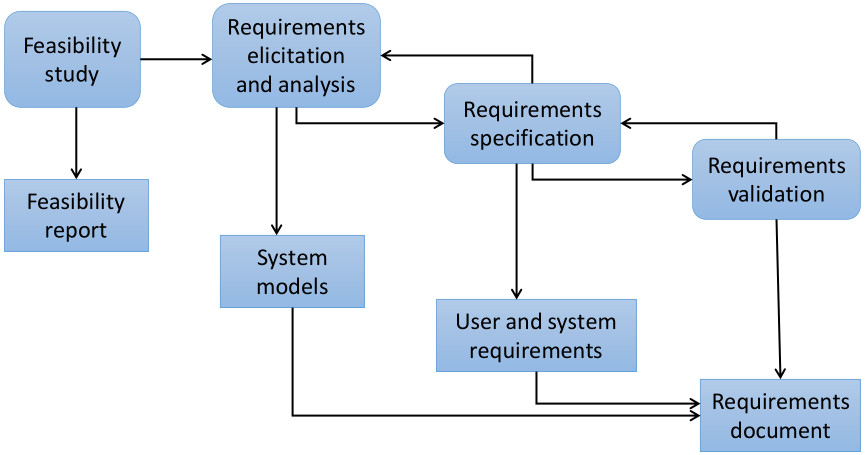
\includegraphics[scale=.3,trim=1cm 1cm 1cm 1cm]{assets/CEN4010_RE_Process.jpg}
\end{figure}
\subsection{Feasibility Studies}
\begin{itemize}
  \item A feasibility study decides whether or not the proposed
system is worthwhile.
  \item A short focused study that checks
  \begin{itemize}
    \item If the system contributes to organizational objectives
    \item If the system can be engineered using current technology \& within budget
    \item If the system can be integrated with other systems that are used
  \end{itemize}
\end{itemize}
\end{multicols}

\vspace{-2em}
\subsection{Elicitation \& analysis}
\begin{itemize}
  \item Involves technical staff working with customers to find out about the application domain, the
services that the system should provide \& the system's operational constraints.
  \item May involve stakeholders: end-users, managers, engineers involved in maintenance, domain experts, trade unions, etc.
\end{itemize}
\textbfr{Problems}
\begin{itemize}
  \item Stakeholders don't know what they really want.
  \item Stakeholders express requirements in their own terms.
  \item Different stakeholders may have conflicting requirements.
  \item Organizational \& political factors may influence the system requirements.
  \item The requirements change during the analysis process; new stakeholders emerge, business env change.
\end{itemize}

\begin{multicols}{2}
\subsection{Requirements validation}
\begin{itemize}
  \item Concerned with demonstrating that requirements define the system that the customer really wants.
  \item Requirements error costs are high so validation is very important
  \begin{itemize}
    \item Fixing requirements error after delivery may cost 100 times the cost of fixing an implementation error.
  \end{itemize}
\end{itemize}
  
\subsection{Requirements checking}
\begin{description}[style=multiline,leftmargin=7em]
  \item [\textr{Validity}] Does system provide functions which best support
the customer's needs?
  \item [\textr{Consistency}] Are there any requirements conflicts?
  \item [\textr{Completeness}] Are all functions required included?
  \item [\textr{Realism}] Can the requirements be implemented given available budget
\& technology
  \item [\textr{Verifiability}] Can the requirements be checked?
\end{description}
\end{multicols}

\begin{multicols}{2}
\subsection{SRS Document Goal}
\noindent The Software Requirements Specification document goal is to serve as a \textbf{template for development}, a low/high level design can be used to understand the system for implementation, enhancement, changes, maintenance, etc.\newline
\vfill\columnbreak
\subsection{SRS Document Structure}
\begin{itemize}
  \item Introduction
  \item Glossary
  \item User requirements definition
  \item System architecture
  \item System requirements specification
  \item System models
  \item System evolution
  \item Appendices
  \item Index
\end{itemize}
\end{multicols}



\chapter{Software Processes}
\section{The Software Process}
A structured set of activities required to develop a software system.\newline
Many different software processes but all involve:
\begin{description}
  \item [Specification] defining what the system should do;
  \item [Design \& implementation] defining the organization of the
system \& implementing the system;
  \item [Validation] checking that it does what the customer wants;
  \item [Evolution] changing the system in response to changing
customer needs.
\end{description}
A software process model is an abstract representation of a process. It presents a description of a process from some particular perspective.

\subsection{Software Process Descriptions}

\subsection{Plan-Driven \& Agile Processes}
\textbf{Plan-Driven processes} are processors where all of the process activities are planned in advance \& progress is measured against this plan. Plan-drive \textbf{can be incremental}, but incremental development usually is agile. In \textbf{Agile processes}, planning is incremental \& it is easier to change the process to reflect changing customer requirements. All agile methods \textbf{use incremental development}, with usually two week sprint cycles \& deliverables. In practice, most practical processes include elements of \textbf{both plan-drive \& agile} approaches. There are no right or wrong software processes.
\begin{description}
  \item [Plan-Driven:] Waterfall Model, Spiral Model
  \item [Agile:] Incremental Development, Scrum, XP, Dynamic Systems Development
\end{description}


\subsection{Software Process vs Software Process Model Q/A}
\begin{description}
  \item [What is a software process?] \ \newline The abstract representation of a process used for development either Plan-Driven or Agile, or a combination
  \item [What is a software process model?] \ \newline The process model used for project documentation \&/or development
  \item [What is the difference?] \ \newline The process is the general approach used for development, \& the model is the actual style \& method, the steps required, for the development process
\end{description}

\section{Software Process Models}
\begin{description}
  \item [The Waterfall model] - Generic 1 \newline Separate \& distinct phases of specification \& development.  \textbf{Plan-driven} model\newline
  \textbf{Good for:} safety critical systems, government projects, large projects developed at many sites
  \item [Incremental development] - Generic 2 \newline Specification, development, \& validation are interleaved. May be \textbf{plan-driven or agile}.\newline
  \textbf{Good for:} business systems, web, distributed applications
  \item [Reuse-based] - Generic 3 \newline The system is assembled from existing components. May be \textbf{plan-driven or agile}.\newline
  \textbf{Good for:} Modifying or replacing existing systems
  \item [Evolutionary] \ \newline Specification \& development are interleaved
  \item [Formal Transformation] \ \newline A mathematical system model is formally transformed to an implementation
  \item [Spiral]
  \item [V shaped]
\end{description}
In practice, most large systems are developed using a process that incorporates elements from all of these models.

\newpage

\subsection{Waterfall Process Model}

% ----------------------------------- COMMENTED OUT----------------------------------------------------
\comment {
\subsubsection{Waterfall Model Documents}
\begin{tabular}{|l|l|}
    \hline
	\thead{Activity} & \thead{Output Documents}\\
    \hline
Requirements analysis & Feasibility study, Outline requirements\\
    \hline
Requirements definition & Requirements document\\
    \hline
System specification & Functional specification, Acceptance test plan \newline Draft user manual\\
    \hline
Architectural design & Architectural specification, System test plan\\
    \hline
Interface design & Interface specification, Integration test plan\\
    \hline
Detailed design & Design specification, Unit test plan\\
    \hline
Coding & Program code\\
    \hline
Unit testing & Unit test report\\
    \hline
Module testing & Module test report\\
    \hline
Integration testing & Integration test report, Final user manual\\
    \hline
System testing & System test report\\
    \hline
Acceptance testing & Final system plus documentation\\
    \hline
  \end{tabular}
}
% ----------------------------------- COMMENTED OUT----------------------------------------------------

\subsubsection{Waterfall Model Phases} 
\begin{description}
  \item [Requirements analysis \& definition] \ \newline
  System’s services, constraints, \& goals established \newline
  System specification
  \item [System \& software design] \ \newline
  \textbf{System Design} allocates requirements to either hardware or software systems. \newline
  \textbf{Software Design} involves identification of fundamental software system abstractions \& their relationships
  \item [Implementation \& unit testing] \ \newline
  Software design is realized as a set of programs \newline
  Unit testing
  \item [Integration \& system testing] \ \newline
  Integration of programs \newline
  Testing
  \item [Operation \& maintenance] \ \newline
  System is installed \& put into practical use \newline
  Maintenance (correcting errors) \newline
  Enhancing system’s services
\end{description}

\subsubsection{Waterfall Model Benefits}
\begin{description}
  \item [Documentation] All aspects are heavily documented
  \item [Rigid project structure] Project structure is well defined \& done in phases
  \item [Advanced planning] Planning is done ahead of other phases like development
  \item [Maintainability] Having lots of documentation leads to a more maintainable system in the long term
  \item [Feature Creep] Limits adding excessive or repeated features that cause delays in development
  \item [Cost/Budget Estimation/Management] Easier \& more accurate control over cost/budget \& estimation/mangement
\end{description}

\subsubsection{Waterfall Model Problems}
\begin{description}
  \item [Heavy Documentation] \ \newline
  There are a lot of documents involved in this model that must be maintained \& updated throughout the life of the project \& into evolution/maintenance
  \item [Difficulty of accommodating change] \ \newline
  The main drawback of the waterfall model is the difficulty of accommodating change after the process is underway.
  \item [Must complete a phase before the next] \ \newline 
  In principle, a phase has to be completed before moving onto the next phase.
  \item [Inability to split up stages] \ \newline
  Inflexible partitioning of project into distinct stages makes it hard to respond to changing requirements.
  \begin{itemize}
    \item Therefore, this model is only appropriate when the requirements are well-understood \& changes will be fairly limited during the design process.
    \item Few business systems have stable requirements.
  \end{itemize}
  \item [Used for large projects] \ \newline
   Mostly used for large systems engineering projects where a system is developed at several sites.
  \begin{itemize}
    \item In those circumstances, the plan-driven nature of the waterfall model helps coordinate the work.
  \end{itemize}
\end{description}

\newpage
\subsection{Incremental Development}
It is based on the \textbf{idea of development in initial implementation, exposing this to user comment \& evolving it through several versions until an adequate system has been developed. Specification, development, \& validation are interleaved} rather than separate, with rapid feedback across activities.

\subsubsection{Incremental Development Benefits}
\begin{description}
  \item [The cost of accommodating changing customer requirements is reduced] \ \newline
  The amount of analysis \& documentation to be redone is much less than is required with waterfall model
  \item [It is easier to get customer feedback on the development work that has to be done] \ \newline
  Customers can comment on the demonstrations of the software \& see how much has been implemented
  \item [More rapid delivery \& deployment of useful software to the customer is possible] \ \newline
  Customers are able to use \& gain value from the software earlier than is possible with a waterfall process.
\end{description}


\subsubsection{Incremental Development Problems}
\begin{description}
  \item [The process is not visible] \ \newline
  Managers need regular deliverables to measure progress. If systems are developed quickly, it is not cost-effective to produce documents that reflect every version of the system.
  \item [System structure tends to degrade as new increments are added] \ \newline
  Unless time \& money is spent on refactoring to improve the software, regular change tends to corrupt its structure\newline
  Incorporating further software changes becomes increasingly difficult \& costly.
\end{description}

\subsection{Reuse-Oriented Software Engineering}
Based on systematic reuse where systems are integrated from existing components or COTS(Commercial-off-the-shelf) systems. Reuse is now the standard approach for building many types of business systems.\newline
\textbf{Process stages:}
\begin{description}
  \item [Component analysis] \
  \begin{itemize}
    \item Given the requirements specification, a search is made for components to implement that specification.
    \item Usually, there is no exact match \& the components that may be used only provide some of the required functionality.
  \end{itemize}
  \item[Requirements modification] \
  \begin{itemize}
  \item During this stage, the requirements are analysed using information about the components that have been discovered.
  \item They are then modified to reflect the available components.
  \item Where modifications are impossible, the component analysis activity may be re-entered to search for alternative solutions.
  \end{itemize}
  \item [System design with reuse] \
  \begin{itemize}
  \item During this phase, the framework of the system is designed or an existing framework is reused.
  \item The designers take into account the components that are reused.
  \end{itemize}
  \item [Development \& integration.] \
  \begin{itemize}
   \item Software that can’t be externally procured is developed, \& the components \& COTS systems are integrated to create the new system.
  \end{itemize}
\end{description}


%--------------------------------------------- Agile ------------------------------------------------
\chapter{Agile Software Development} 
\section{Agile Development Methods Umbrella}
\noindent Scrum, Adaptive Software Development, Feature Driven Development, Lean, Kabanzi Framework, eXtreme Programming (XP), Scrumban, Crystal, Kanban, Dynamic Systems Development Method (DSDM) Agile Unified Process (AUP), Pragmatic Programming

\subsection{Agile Techniques}
\noindent Continuous Integration, Test Driven Development, Pair Programming, Agile Change Management, Agile Modeling, Release Planning

\subsection{Agile Methods}
\noindent The aim of agile methods is to reduce overheads in the software process (e.g. by limiting documentation) \& to be able to respond quickly to changing requirements without excessive rework.
\begin{itemize}
  \item Focus on the code rather than the design
  \item Are based on an iterative approach to software development
  \item Are intended to deliver working software quickly \& evolve this quickly to meet changing requirements
  \item Agile methods are incremental development methods
  \begin{itemize}
    \item Increments are small
    \item New releases of the systems are created an made available to customer ever 2 or 3 weeks
  \end{itemize}
  \item Involve customers in the development process to get rapid feedback on changing requirements
  \item Minimize documentation by using informal communications rather than formal meetings with written documentations.
\end{itemize}

\section{Agile Manifesto}
\noindent Stated in 2001, By Kent Beck \& 16 other software developers\newline

\noindent We are uncovering better ways of developing software by doing it \& helping others do it. Through this work we have come to value:\newline
\indent\textr{Individuals \& interactions} \textg{over processes \& tools} \newline
\indent\textr{Working software} \textg{over comprehensive documentation} \newline
\indent\textr{Customer collaboration} \textg{over contract negotiation}\newline
\indent\textr{Responding to change} \textg{over following a plan}\newline
That is, while there is value in the items on the \textbfg{right}, we value items on the \textbfr{left} more.\newline

\noindent For the process, the 5 framework activities are still the same; communication, planning, modeling, construction, \& deployment. For the work product, an operational "software increment" delivered to the customer on the appropriate commitment date.

\section{The Principles of Agile Methods}
\begin{description}[style=multiline,leftmargin=12em]
  \item [Customer involvement] Customers should be closely involved throughout the development process. Their role is provide \& prioritize new system requirements \& to evaluate the iterations of the system.
  \item [Incremental delivery] The softare is developed in increments with the customer specifying the requirements to be included in each increment
  \item [People not process] The skills of the development team should be recognized \& exploited. Team members should be left to develop their own ways of working without prescriptive processes.
  \item [Embrace change] Expect the system requirements to change \& so design the system to accommodate these changes.
  \item [Maintain simplicity] Focus on simplicity in both the software being development \& in the development process. Wherever possible, actively work to eliminate complexity from the system.
\end{description}

\newpage
\section{Agile Method Applicability}
\begin{itemize}
  \item Product development where a software company is developing \textg{a small or medium-sized} product for sale.
  \item \textg{Custom system development} within an organization, where there is a clear commitment from the customer to become involved in the development process \& where there are not a lot of external rules \& regulations that affect the software.
  \item Because of their focus on small, tightly-integrated teams, there are problems in scaling agile methods to large systems.
\end{itemize}  
  
\section{Plan-Drive \& Agile Development}
\vspace{-1em}
\begin{multicols}{2}
\noindent\textbf{Plan-Driven Development}
\begin{itemize}
  \item A plan-driven approach to software engineering is based around separate development stages with the outputs to be produced at each of these stages planned in advance.
  \item Not necessarily waterfall model $-$ plan-drive, incremental development is possible
  \item Iteration occurs within activities
\end{itemize}  
\textbf{Agile Development}
\begin{itemize}
  \item Specification, design, implementation \& testing are interleaved \& the outputs from the development process are decided through a process of negotiation during software development process.
\end{itemize}
\begin{figure}[H]
\centering
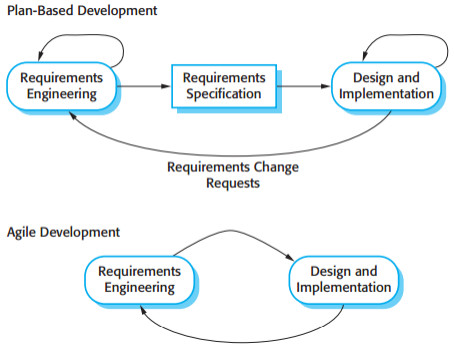
\includegraphics[scale=.5,trim=1cm 1cm 1cm 1cm]{assets/CEN4010_Agile_Plan_Driven.jpg}
\end{figure}
\end{multicols}

\section{Extreme Programming}
\vspace{-1em}
\begin{multicols}{2}
\noindent The best-known \& most widely used agile method. Extreme Programming (XP) takes an 'extreme' approach to iterative development.
\begin{itemize}
  \item New versions may be built several times per day
  \item Increments delivered to customers every 2 weeks
  \item All tests must be successfully executed when new code is integrated into the system.
  \item All tests must be run for every build \& the build is only accepted if tests run successfully.
  \item Requirements are expressed as scenarios (called use stories), which are implemented directly as a series of tasks.
  \item Programmers work in pairs \& develop tests for each task before writing the code.
  \item Short time gap between releases of the system, with small releases
\end{itemize}
\begin{figure}[H]
\centering
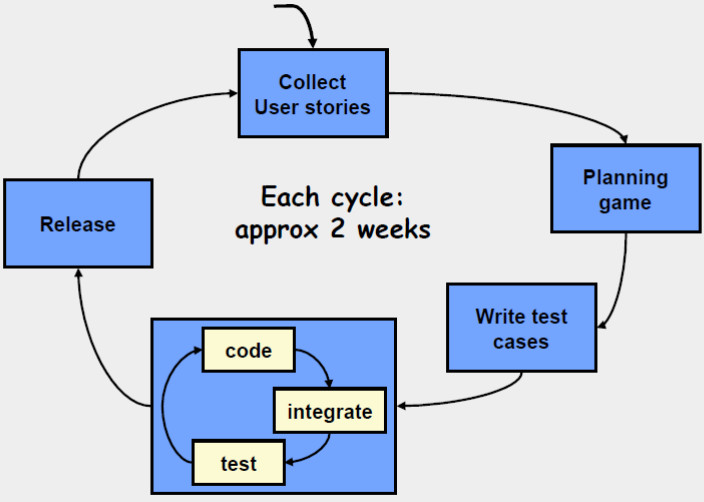
\includegraphics[scale=.25,trim=1cm 1cm 1cm 1cm]{assets/CEN4010_Agile_XP.jpg}
\end{figure}
\begin{figure}[H]
\centering
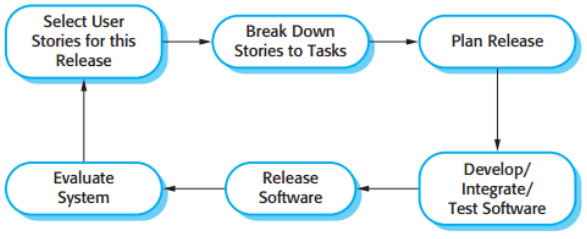
\includegraphics[scale=.35,trim=1cm 1cm 1cm 1cm]{assets/CEN4010_Agile_XP_Release_Cycle.jpg}
\end{figure}
\end{multicols}

\section{XP \& Agile Principles}
\begin{description}[style=multiline,leftmargin=12em]
  \item [\textg{Incremental development}] is supported through small, frequent system releases.
  \item [\textg{Customer Involvement}] means full-time customer engagement with the team.
  \item [\textg{People, not process}] are supported through pair programming, collective ownership \& a process that avoids long working hours.
  \item [\textg{Change}] supported through regular system releases.
  \item [\textg{Maintaining Simplicity}] through constant refactoring of code
\end{description}

\newpage
\section{Extreme Programming Practices}
\begin{description}[style=multiline,leftmargin=12em]
  \item [Incremental planning] Requirements are recorded on story cards \& the stories to be included in a release are determined by the \textr{time available} \& their \textr{relative priority}. The Developers break these stories into development 'Tasks'
    \item [Small releases] Minimal useful set of functionality that provides business value is developed first.\newline
    Releases of the system are frequent \& incrementally add functionality to first release.
  \item [Simple design] Enough design is carried out to meet the current requirements \& no more.
  \item [Test-first development] An automated unit test framework is used to write tests for a new piece of functionality before that functionality itself is implemented.
  \item [Refactoring] All developers are expected to refactor the code continuously as soon as possible code improvements are found. This keeps the code simple \& maintainable.
  \item [Pair programming] developers work in pairs, checking each other's work \& providing the support to always do a good job.
  \item [Collective ownership] The pairs of developers work on all areas of the system, so that no islands of expertise develop \& all the developers take responsibility for all of the code. \textr{Anyone can change anything.}
  \item [Continuous integration] As soon as the work on a task is complete, it is integrated into the whole system. After any such integration, all the unit tests in the system must pass.
  \item [Sustainable pace] Large amounts of overtime are not considered acceptable as the net effect is often to reduce code quality \& medium term productivity.
  \item [On-site customer] A representative of the end-user of the system (the customer) should be available full time for the use of XP team. In an extreme programming process, the customer is a member of the development team \& is responsible for bringing system requirements to the team for implementation.
\end{description}

\section{Requirements Scenarios}
\noindent In XP, \textg{a customer or user} is part of the XP team \& is responsible for making decisions on requirements. User requirements are expressed as scenarios or user stories. These are written on cards \& the development team break them down into implementation tasks. These tasks are the basis of \textg{schedule \& cost estimates}. The \textg{customer} chooses the stories for inclusion in the next release based on their \textg{priorities} \& the \textg{schedule estimates}.


\section{XP \& Change}
\noindent Conventional wisdom in software engineering is to design for change. It is worth spending time \& effort anticipating changes as this reduces costs later in the life cycle. XP, however, maintains that this is not worthwhile as changes cannot be reliably anticipated. Rather, it proposes constant code improvement(refactoring) to make changes easier when they have to be implemented.

\section{Refactoring}
\noindent Programming team look for possible software improvements \& make these improvements even when there is no immediate need for them. This improves the \textg{understandability} of the software \& so reduces the need for documentation. Changes are easier to make because the code is well-structured \& clear. However, some changes require architecture refactoring \& that is much more expensive.\newline

\noindent \textbf{Definition:} Refactoring modifies software to improve its readability, maintainability, \& extensibility without changing what it actually does. (External behavior does not change, internal structure is improved)\newline

\noindent The goal of refactoring is \textbf{NOT} to add new functionality. The goal of refactoring is to make code easier to maintain in the future. This supports:
\begin{itemize}
  \item Program Comprehension
  \item Source Code Analysis
  \item Software Maintenance
  \item Software Traceability
\end{itemize}

\newpage
\subsection{Examples of Refactoring}
\noindent
\begin{itemize}
  \item \textg{Re-organization} of a class hierarchy to remove duplicate code.
  \item Tidying up \& \textg{renaming} attributes \& methods to make them easier to understand
  \item The \textg{replacement} of inline code with calls to methods that have been included in a program library.
\end{itemize}

\subsection{Danger of refactoring}
\noindent Refactoring \textbf{CAN} introduce problems, because anytime you modify, software you may introduce bugs! Refactoring adds risk \& is expensive.

\subsection{Motivation}
\noindent We refactor because getting the design right the first time is hard \& you get many benefits from refactoring.
\begin{itemize}
  \item Code size is often reduced
  \item Confusing code is restructured into simpler code
  \item Both of these greatly improve maintainability! Which is required because requirements always change!
\end{itemize}

\subsection{Testing in XP}
\noindent Testing is central to XP \& XP has developed an approach where the program is tested after every change has been made. XP Testing features:
\begin{itemize}
  \item Test-first development
  \item Incremental test development from scenarios
  \item User involvement in test development \& validation
  \item The use of automated testing frameworks
\end{itemize}

\section{Test-First Development}
\noindent Writing tests before code \textg{clarifies the requirements} to be implemented. Tests are \textg{written as programs} rather than data so that they can be executed automatically. The tests includes a check that it has executed correctly. Usually relies on a testing framework such as Junit, Check/libCheck, etc. All previous \& new tests are run automatically when new functionality is added, thus checking that new functionality has not introduced errors.

\subsection{Customer Involvement}
\begin{itemize}
  \item The role of the customer in the testing process is to help develop \textg{acceptance tests} for the stories that are to be implemented in the next release of the system.
  \item The customer who is part of the team writes tests as development proceeds.
  \item All new code is therefore validated to ensure that it is what the customer needs.
\end{itemize}

\subsection{Test Automation}
\noindent Test automation means that tests are written as executable components before the task implemented.
\begin{itemize}
  \item An automated test framework (e.g. Junit, Check, etc) is a system that makes it easy to write executable tests \& submit a set of tests for execution.
\end{itemize}
As testing is automated, there is always a set of tests that can be quickly \& easily executed.
\begin{itemize}
  \item Whenever any functionality is added to the system, the tests can be run \& problems that the new code has introduced can be caught immediately.
\end{itemize}

\subsection{XP Testing difficulties}
\begin{itemize}
  \item Incomplete tests - do not check for all possible exceptions that may occur
  \item Some tests can be very difficult to write incrementally
  \item It is difficult to judge the completeness of a set of tests
  \item It supports the idea of collective ownership \& responsibility for the system.
  \item It acts as an informal review process because each line of code is looked at by at least two people.
  \item It helps support refactoring, which is a process of software improvement.
\end{itemize}

\section{Pair Programming}
\noindent In XP, programmers work in pairs, sitting together to develop code. This helps develop a common ownership of code \& spreads knowledge across the team. It serves as an informal review process as each line of code is looked at by more than 1 person. It encourages refactoring as the whole team an benefit from this. Measurements suggest that development productivity with pair programming is similar to that of two people working independently.

\newpage
\section{SCRUM}
\noindent The SCRUM approach is a general agile method but its focus is on managing iterative development rather than specific agile practices. These are three phases in scrum.
\begin{multicols}{2}
\begin{enumerate}
  \item The initial phase is an \textbfv{outline planning phase} where you establish the general objectives for the project \& \textbfv{design the software architecture}.
  \item This is followed by a series of \textbfv{spring cycles}, where each cycle develops an \textbfv{increment} of the system.
  \item The \textbfv{project closure} phase wraps up the project, completes required documentation such as system hep frames \& user manuals \& assesses the lessons learned from the project.
\end{enumerate}

\subsection{The SCRUM Process}
\begin{figure}[H]
\centering
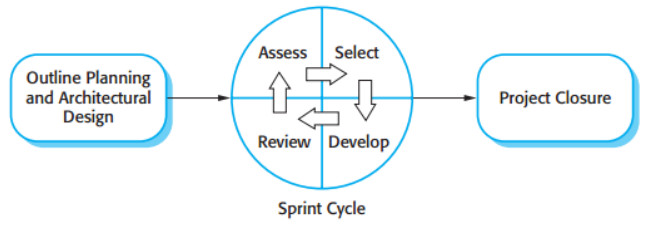
\includegraphics[scale=.4,trim=1cm 1cm 1cm 1cm]{assets/CEN4010_Scrum_Process.jpg}
\end{figure}
\end{multicols}

\subsection{The SCRUM Sprint Cycle}
\begin{itemize}
  \item \textbfv{Sprints are fixed length, normally 2-4 weeks.} They correspond to the development of a release of the system in XP.
  \item The starting point for \textbfv{planning} is the product backlog, which is the list of work to be done on the project.
  \item During the \textbfv{assessment phase}, this is reviewed, \& priorities \& risks are assigned.
  \item The \textbfv{selection} phase involves all of the project team who work with the customer to select the features \& functionality to be developed during the sprint.
  \item Once these are agreed, the team organize themselves \textbfv{develop} the software.
  \item During this state the team is isolated from teh customer \& the organization, with all communication channeled through the so-called \textbfg{'Srum master'}
  \item \textg{The role of the Scrum master is to protect the development team from external distractions.}
  \item At the end of the sprint, the work is \textbfv{reviewed} \& presented to stakeholders. The next spring cycle begins.
\end{itemize}
\begin{figure}[H]
\centering
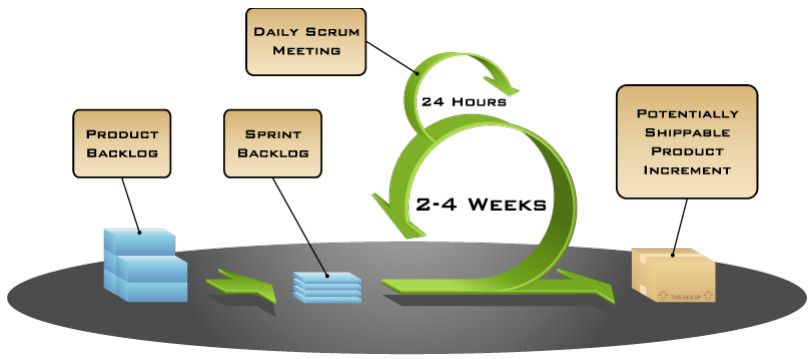
\includegraphics[scale=.5,trim=1cm 1cm 1cm 1cm]{assets/CEN4010_Scrum_Overview.jpg}
\end{figure}

\subsection{SCRUM Benefits}
\begin{multicols}{2}
\noindent Rising \& Janoff discussed successful use of SCRUM in a telecommunications SDE
\begin{itemize}
  \item The product is broken down into a set of manageable \& understandable chunks.
  \item Unstable requirements do not hold up progress.
  \item The whole team had visibility of everything \& consequently team communication is improved.
  \item Customers see on-time delivery of increments \& gain feedback on how the product works.
  \item Trust between customers \& developers is established \& a positive culture is created in which everyone expect the project to succeed.
\end{itemize}
\vfill\columnbreak
\begin{figure}[H]
\centering
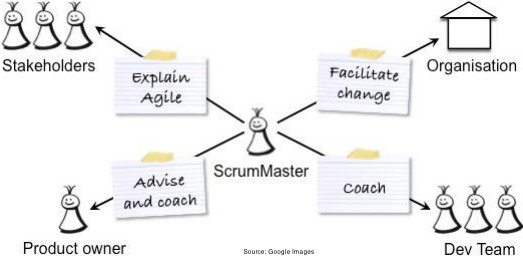
\includegraphics[scale=.4,trim=1cm 1cm 1cm 1cm]{assets/CEN4010_Scrum_Cycle.jpg}
\end{figure}
\end{multicols}


%------------------------------------- An Ounce of Prevention ----------------------------------

\renewcommand\thechapter{A1}
\chapter{An Once of Prevention}
\noindent\textbf{Involve end users as early as possible}\newline
Several studies have found that end-user involvement is a key to stable requirements \& software project success.\newline

\noindent\textbf{Create a throwaway prototyping}\newline
Create throwaway UI prototype code; put the prototype in front of real end users. Get feedback. Revise the prototype until the user is excited about the system. Then build the system. This approach is correlated with good requirements stability \& low system cost.\newline

\noindent\textbf{Deliver the software incrementally instead of all at once}\newline
Write production code for a small amount of the system. Put that functionality in front of the user. Revise the requirements, design, \& code until the user is excited about the system. This approach does not entirely eliminate the defect-cost-increase dynamic, but it shortens the feedback loop from requirements to user feedback in a way that reduces the number of downstream dependences that will be based on erroneous upstream work. This sort of incremental delivery approach is correlated with high user satisfaction \& lower total development costs.\newline

\noindent\textbf{Conduct a requirements workshop}\newline
Fast requirements elicitation techniques such as JAD sessions have been found to be an effective way to shorten the time required to collect accurate requirements while simultaneously reducing requirements volatility downstream.\newline

\noindent\textbf{Perform use case analysis}\newline
Rather than being satisfied with users? first explanation of what they want a system to do, examine the expected usage patterns of the system to better understand the users real needs.\newline

\noindent\textbf{Create the user manual first}\newline
Some organizations have had good success creating their user manuals as a substitute for or supplement to a traditional requirements specification. End users seem to be better able to understand the contents of a user manual than a traditional requirements specification, \& requirements elicitation goes more smoothly

%------------------------------------- Spiral Model ----------------------------------

\renewcommand\thechapter{A2}
\chapter{Spiral Model}
\noindent\textbf{Traditional software process models} were \textbf{discouraging more effective approaches} to software development such as prototyping \& software reuse.\newline

\noindent The \textbf{major distinguishing feature} of the spiral model is that it creates a \textbf{risk-driven approach} to the software process rather than a primarily document-driven or code-driven process. It \textbf{incorporates} many of the \textbf{strengths of other models} \& \textbf{resolves} many of their \textbf{difficulties}

\section{Process Model vs Method}
\noindent The primary functions of a software process model are to \textbf{determine the order of the stages} involved in software development \& evolution \& to establish the transition criteria for progressing from one stage to the next.\newline

\noindent A process model differs from a software method (often called a methodology) in that a method’s primary focus is on \textbf{how to navigate through each phase}

\section{Pursuing Stages in the wrong order}
\noindent These projects are examples of how \textbf{waterfall model} projects have come to grief by pursuing stages in the wrong order. \textbf{Evolutionary development} projects have come to grief by pursuing stages in the wrong order

\section{Tables became standard}
\noindent It is also interesting to note that the form of Tables I, 2, \& 3 was originally developed for presentation purposes, but subsequently became a standard \textbf{"spiral model template"} used on later projects.

\section{Benefits}
\begin{itemize}
  \item Its \textbf{risk-avoidance} features will generally \textbf{avoid the difficulties} of the other models
  \item It focuses early \textbf{attention} on options involving the \textbf{reuse of existing software}
  \item It accommodates preparation for \textbf{life-cycle evolution, growth, \& changes} of the software product
  \item It provides a mechanism for incorporating \textbf{software quality objectives} into software product development
  \item It focuses on \textbf{eliminating errors \& unattractive alternatives} early
  \item For each sources of project activity \& resource expenditure, answers the question, \textbf{"How much is enough?"}
  \item It \textbf{does not involve separate approaches} for software \textbf{development \& enhancement (or maintenance)}.
  \item It provides a \textbf{viable framework} for \textbf{integrated hardware-software} system development.
\end{itemize}

\section{Drawbacks}
\noindent The three primary challenges involve \textbf{matching to contract software}, \textbf{relying on risk-assessment expertise}, \& the need for \textbf{further elaboration of spiral model steps}.


\end{document}
